\documentclass{beamer}

\usetheme{default}
\usepackage[utf8]{inputenc}

\setbeamertemplate{footline}[frame number]
\setbeamertemplate{frametitle}[default][center]

\mode<presentation>{
\usetheme{Dresden}
%\setbeamercovered{transparent}
\usecolortheme{seagull}
}

\setbeamertemplate{headline}{}

\definecolor{peeblue}{RGB}{1,123,165}
\setbeamercolor*{palette primary}{fg=black,bg=peeblue!80}
\setbeamercolor*{palette secondary}{fg=black,bg=peeblue!80!gray!80}
\setbeamercolor*{palette tertiary}{fg=black,bg=peeblue!100}
\setbeamercolor*{palette quaternary}{fg=black,bg=peeblue!110}

\usebackgroundtemplate
{%
    \begin{picture}(210,40)(-5,2)
    
\includegraphics[width=0.07\paperwidth,keepaspectratio]{imgs/pee-logo-short.png}
    \end{picture}%
}

 \AtBeginSection[]
  {
    \begin{frame}
      \centering
      \huge\insertsectionhead
    \end{frame}
  }

\title{Técnicas de Regularização em Aprendizado Profundo}
\author{Autor da Apresentação}
\date{\today}

\institute
{
  Universidade Federal do Rio de Janeiro\\
  UFRJ/COPPE/PEE
}


% Let's get started
\begin{document}

{
\usebackgroundtemplate{
    \begin{picture}(210,55)(-5,0)
    
\includegraphics[height=0.14\paperwidth,keepaspectratio]{imgs/pee-logo.png}
    \end{picture}%
    \begin{picture}(210,55)(-28,2)
    
\includegraphics[height=0.14\paperwidth,keepaspectratio]{imgs/coppe-logo.pdf}
    \end{picture}
}
\begin{frame}
  \bigskip\bigskip\bigskip\bigskip
  \titlepage
\end{frame}
}

\begin{frame}{Agenda}
  \tableofcontents
\end{frame}

\section{Introdução}

\begin{frame}{Definição}
\begin{quote}
``Any modification we make to a learning algorithm that is intended to reduce its generalization error but not its training error.''
\end{quote}
\vspace{0.5cm}
\raggedleft
--- Goodfellow et al. Deep Learning
\end{frame}

\begin{frame}{O Problema do Overfitting}
\centering
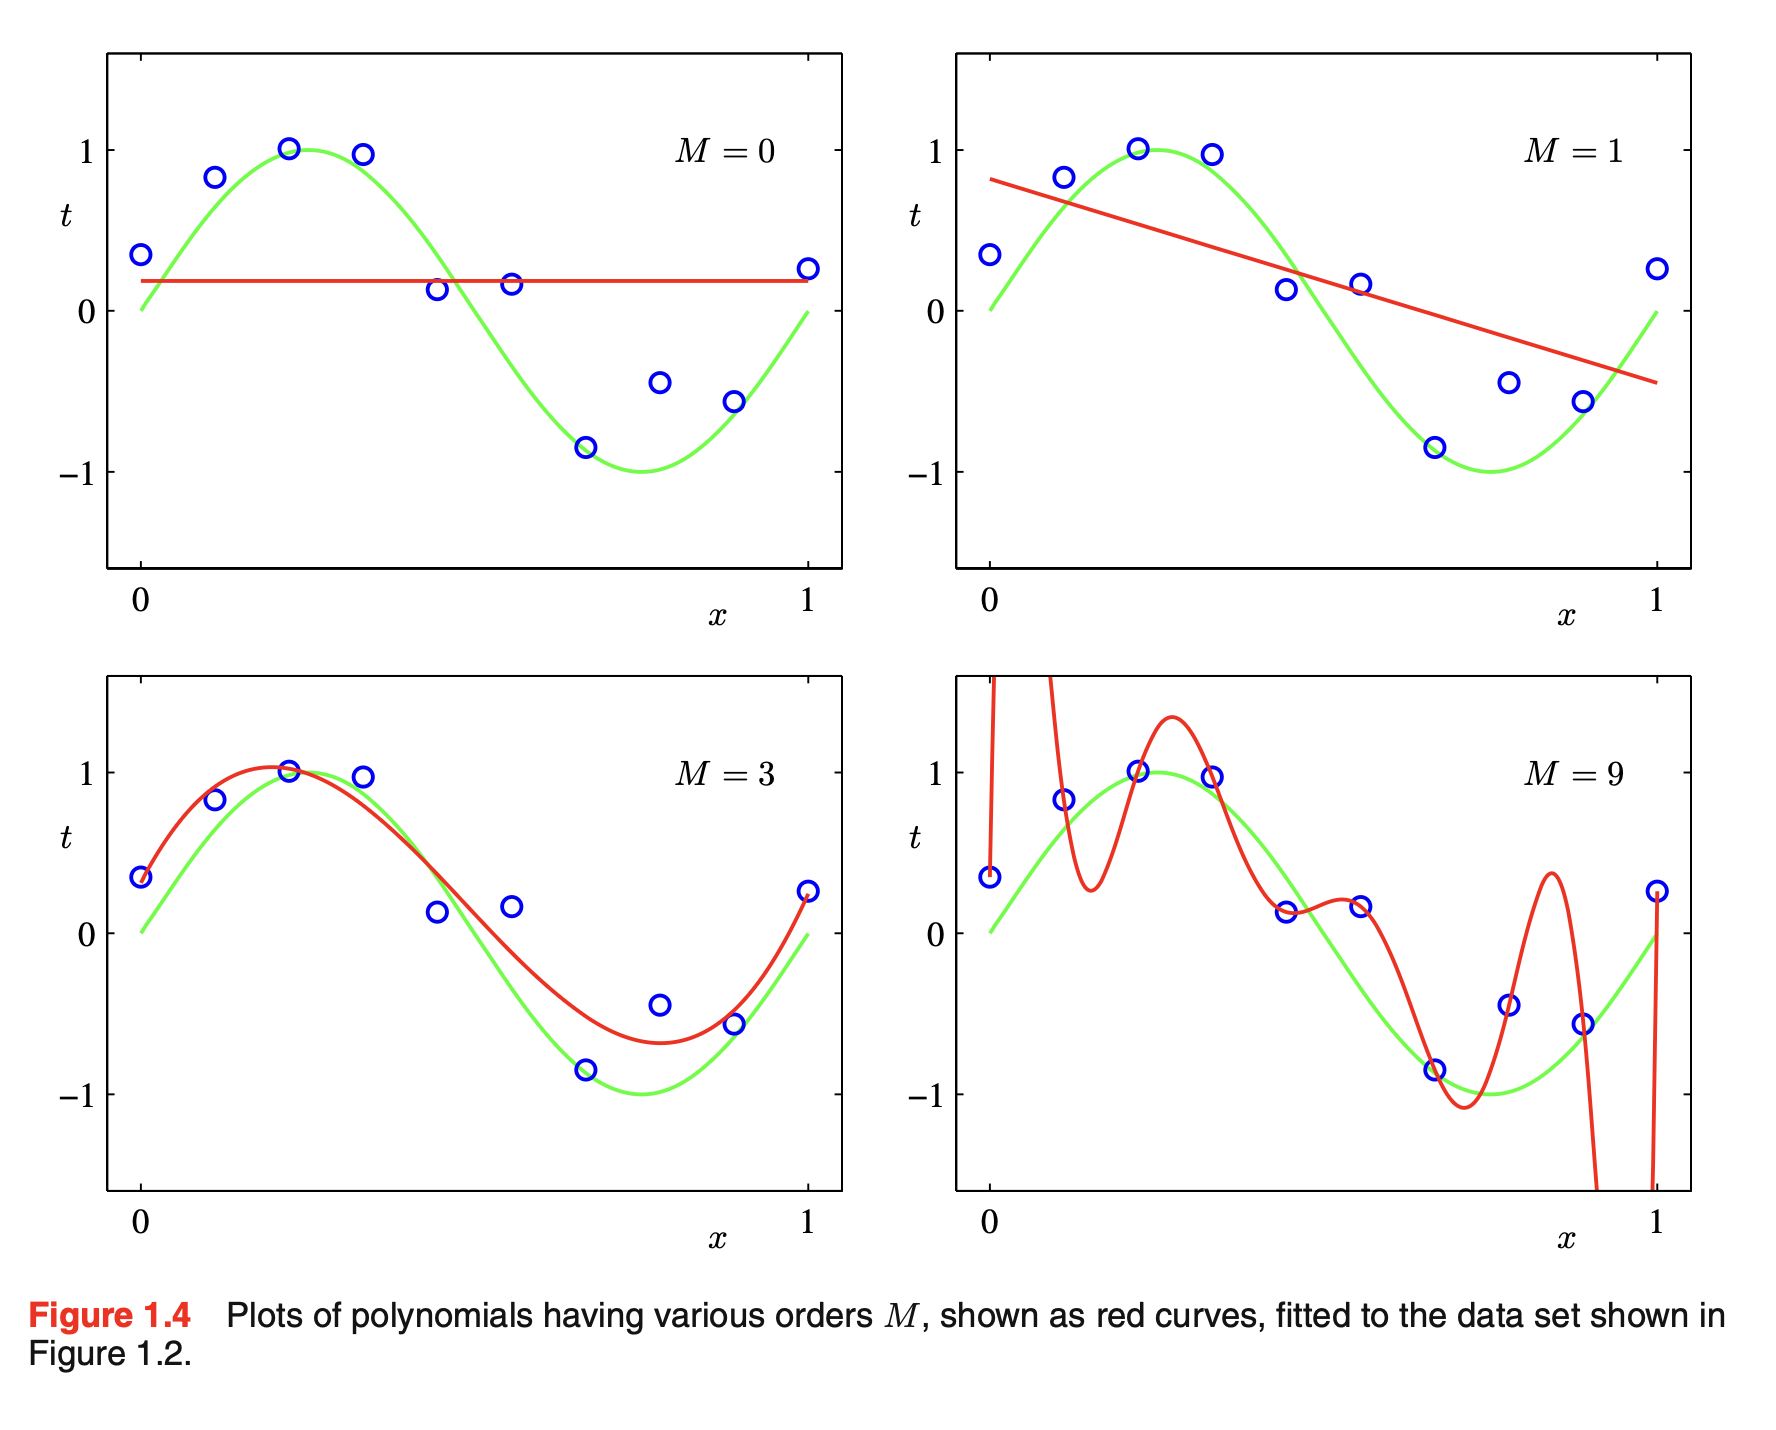
\includegraphics[width=\textwidth,height=0.8\textheight,keepaspectratio]{imgs/bishop_example/1.png}
\end{frame}

\begin{frame}
\centering
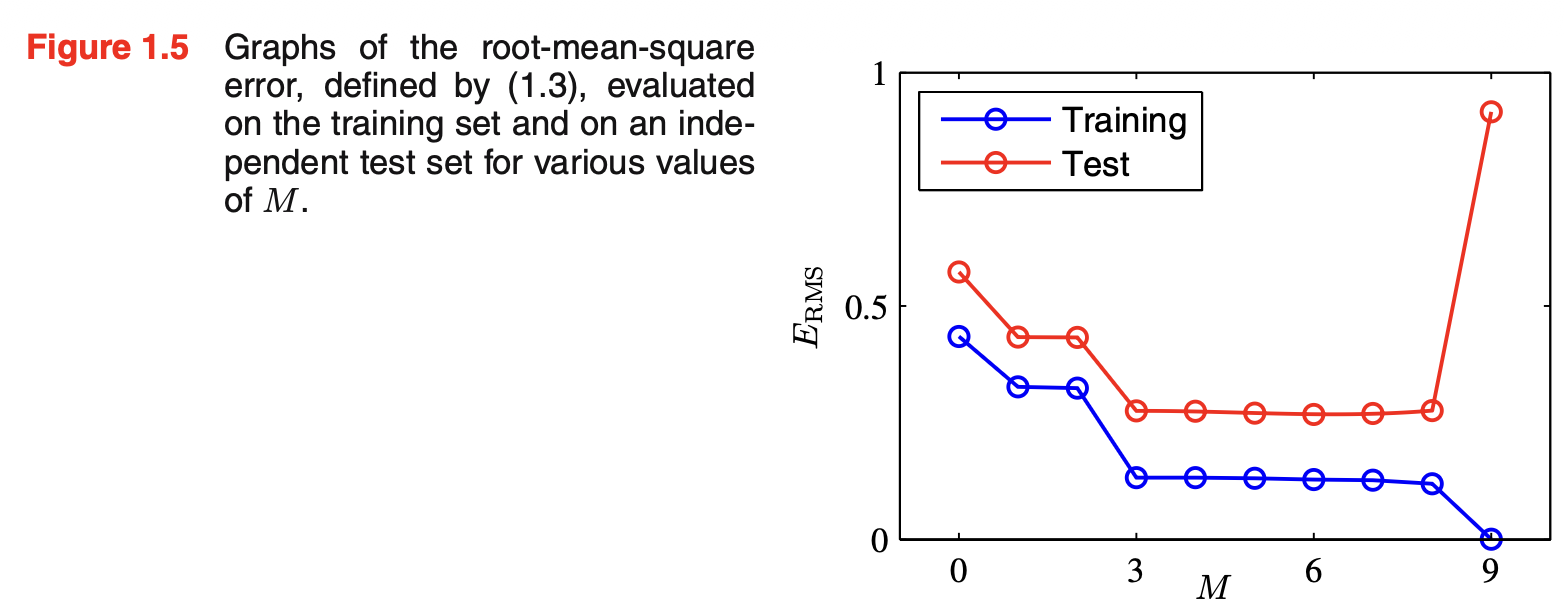
\includegraphics[width=\textwidth,height=0.8\textheight,keepaspectratio]{imgs/bishop_example/2.png}
\end{frame}

\begin{frame}{Alternativa 1: aumentar a quantidade de dados no treinamento}
\tiny{\textit{"The best way to make a machine learning model generalize better is to train it on
more data. Of course, in practice, the amount of data we have is limited."} --- Goodfellow et al., \textit{Deep Learning}}
\centering
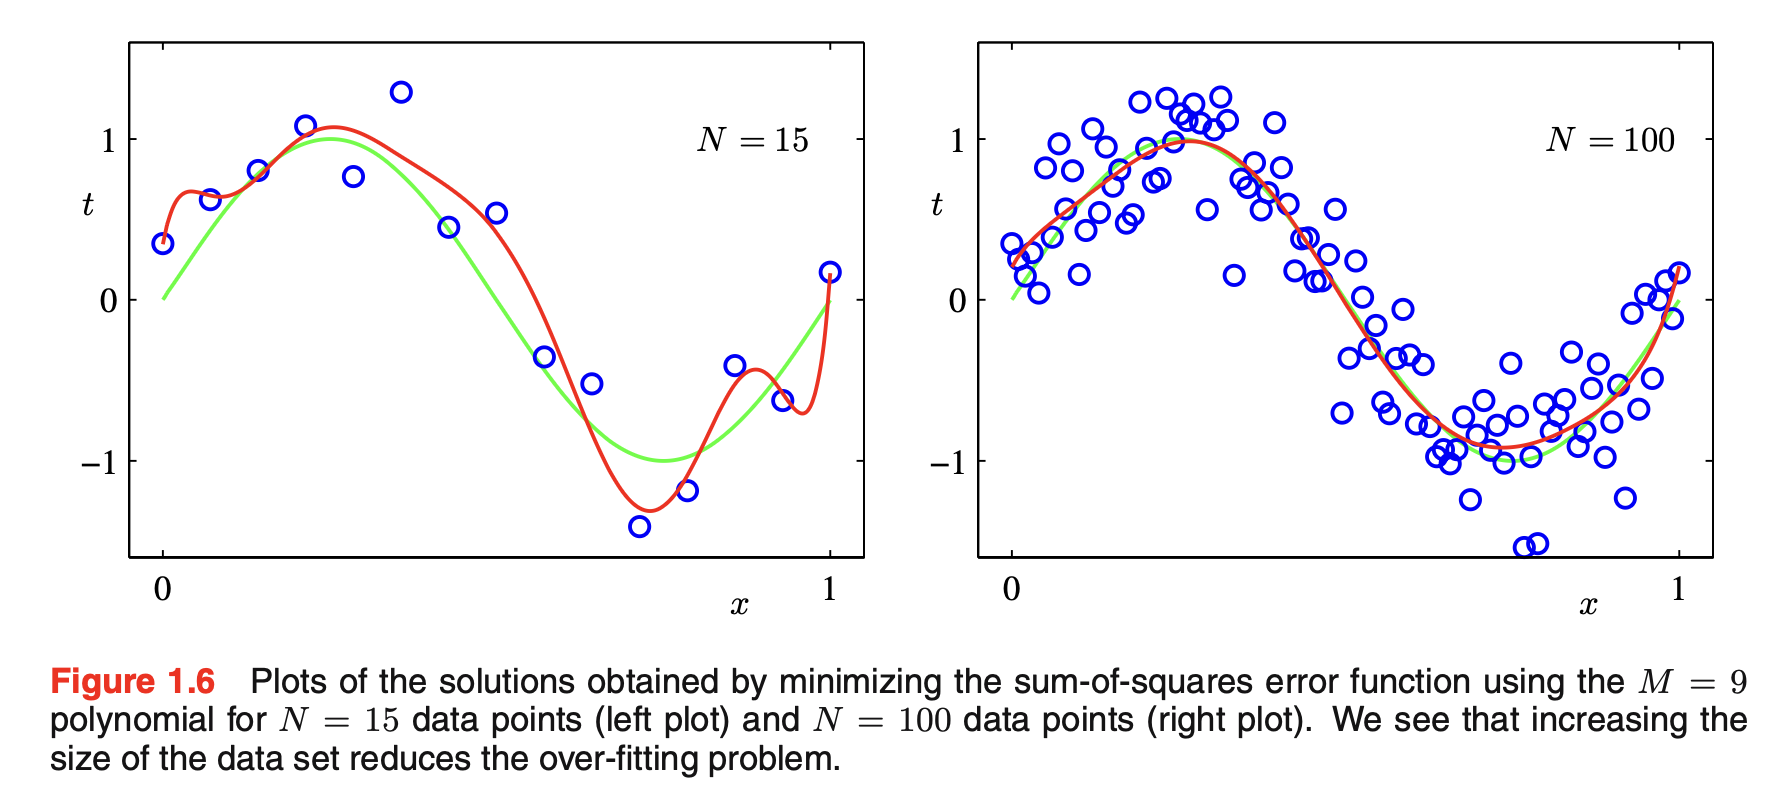
\includegraphics[width=\textwidth,height=0.8\textheight,keepaspectratio]{imgs/bishop_example/3.png}
Nem sempre é possível. Ex: Experimento genético com 500 camundongos, 20000 a 25000 genomas
\end{frame}

\begin{frame}{Alternativa 2: aplicar regularização}
\centering
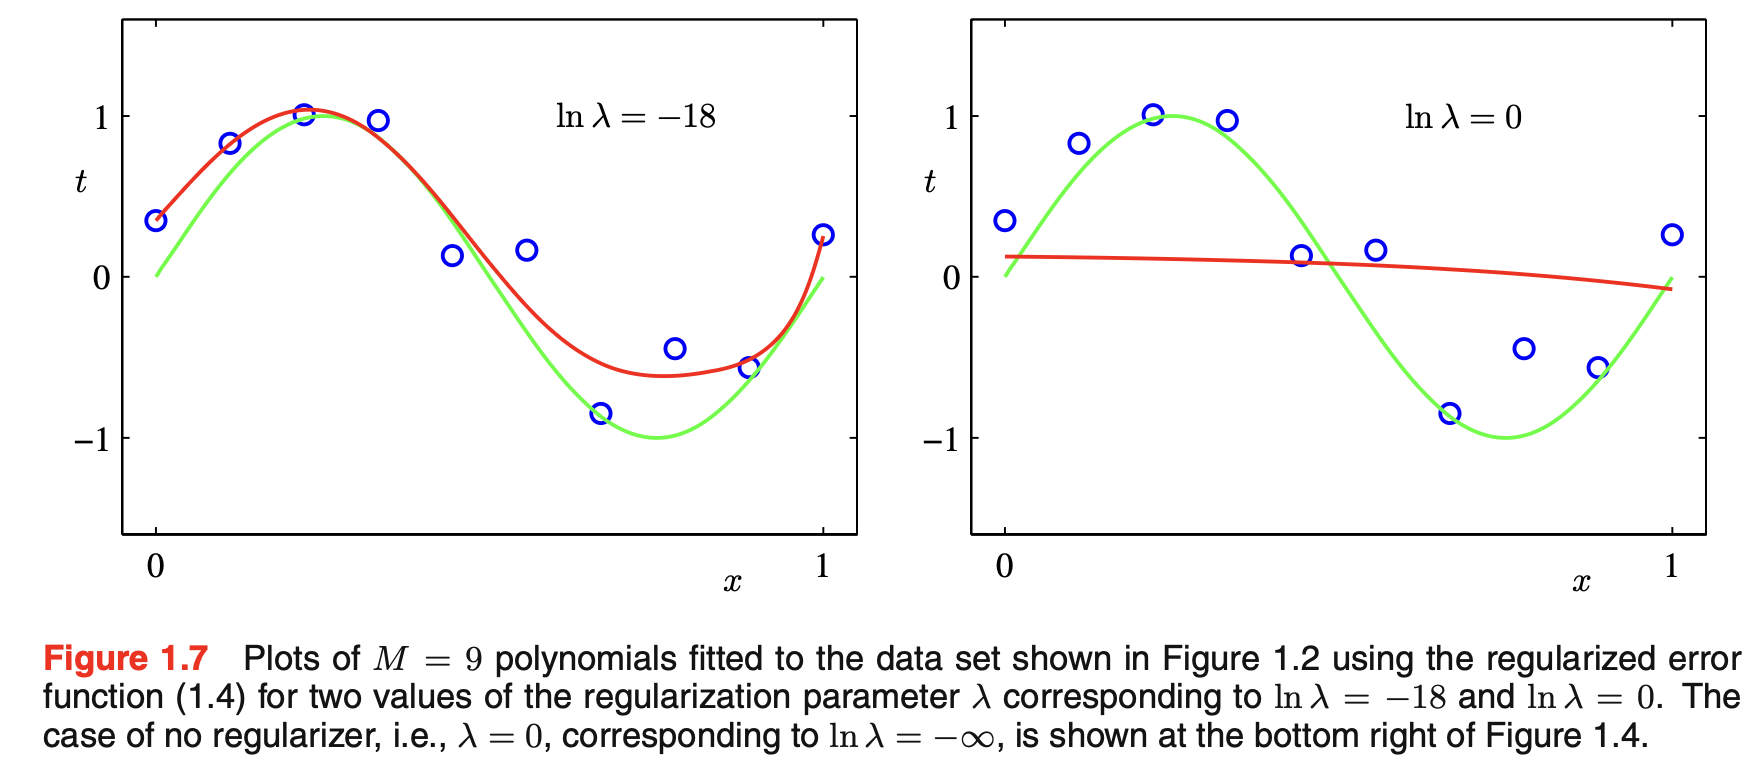
\includegraphics[width=\textwidth,height=0.8\textheight,keepaspectratio]{imgs/bishop_example/4.png}
\end{frame}

\begin{frame}
\centering
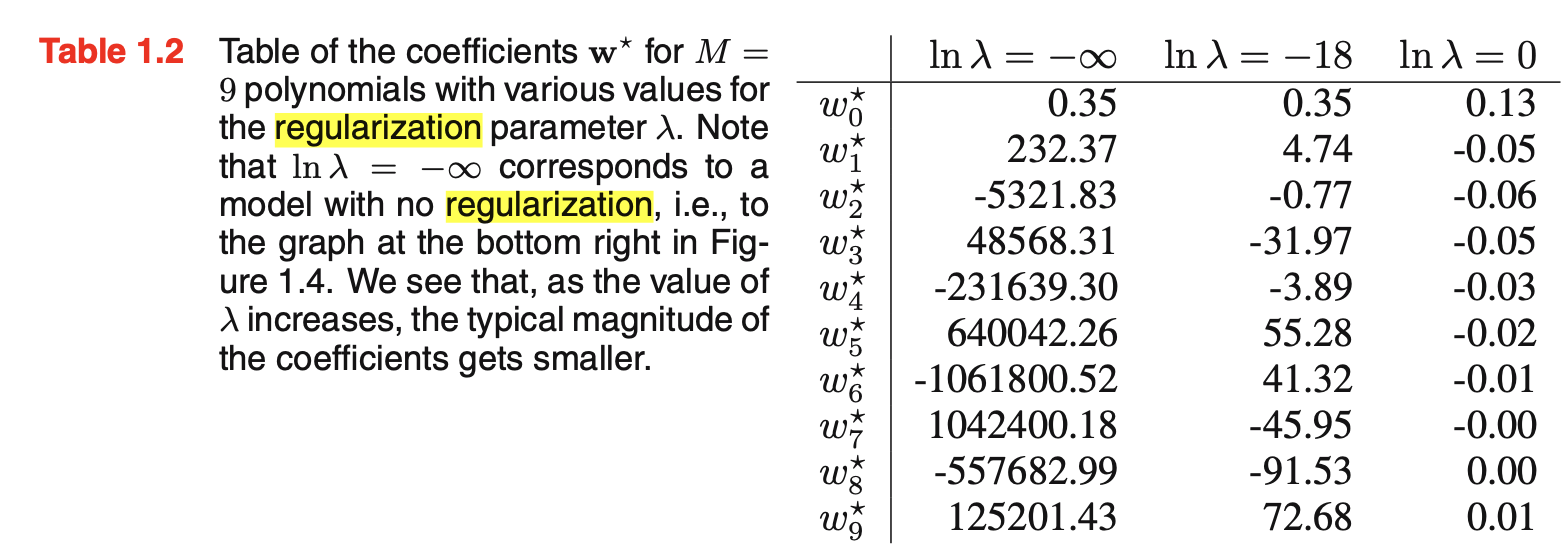
\includegraphics[width=\textwidth,height=0.8\textheight,keepaspectratio]{imgs/bishop_example/5.png}
\footnotesize{Na prática, o valor de $\lambda$ é obtido pela validação cruzada.}
\end{frame}

\section{Otimização com Restrições}

\begin{frame}{Penalização da Norma dos Parâmetros}
\begin{columns}[T]
\begin{column}{0.5\textwidth}
\begin{block}{Regularização L1}
\vspace{0.3cm}
{\tiny
$$\mathcal{L}(\theta) = \frac{1}{N}\sum_{i=1}^{N}\text{Custo}(y_i, f_\theta(x_i)) + \lambda||\theta||_1$$
}
\vspace{0.5cm}
- Pesos esparsos

- \textbf{exatamente zero}
\vspace{0.3cm}
\end{block}
\end{column}

\begin{column}{0.48\textwidth}
\begin{block}{Regularização L2}
\vspace{0.3cm}
{\tiny
$$\mathcal{L}(\theta) = \frac{1}{N}\sum_{i=1}^{N}\text{Custo}(y_i, f_\theta(x_i)) + \lambda||\theta||_2^2$$
}
\vspace{0.5cm}
- Pesos pequenos

- \textbf{nunca exatamente zero}
\vspace{0.3cm}
\end{block}
\end{column}
\end{columns}
\tiny{\begin{quote}
    \textit{"Regularization terms of the form (above) encourage the model weights to have a smaller magnitude and hence introduce a bias towards functions that vary more slowly with changes in the inputs."} --- Bishop et al., \textit{Deep Learning}
\end{quote}}
\end{frame}


\begin{frame}{Interpretação Geométrica}
\centering
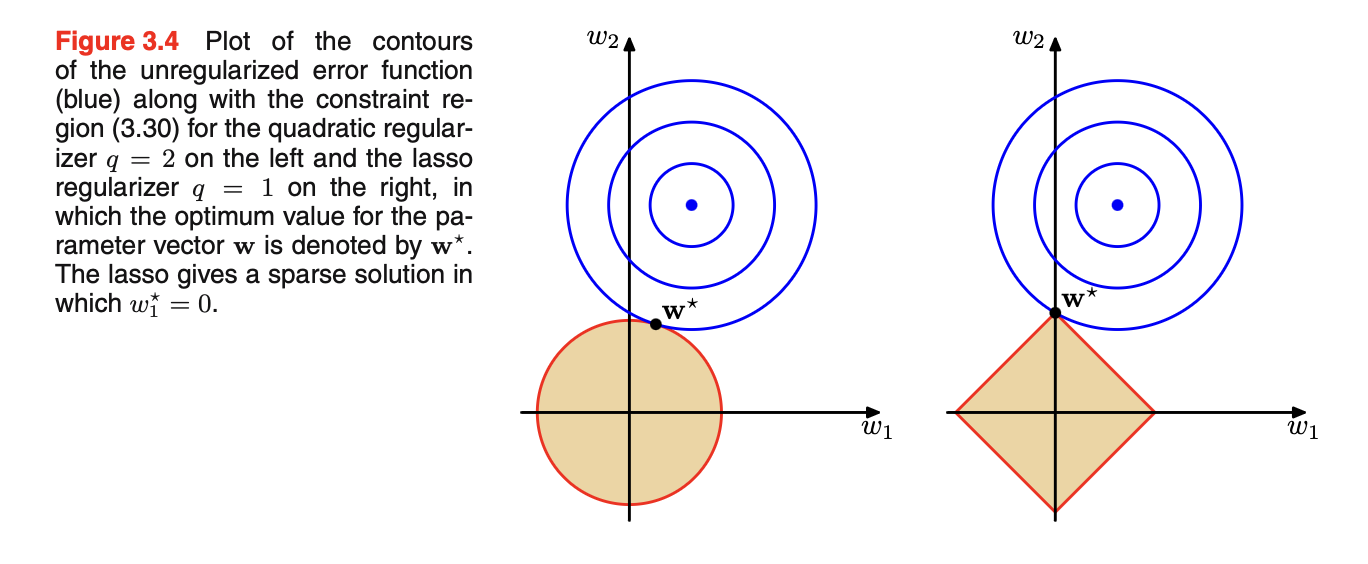
\includegraphics[width=\textwidth,height=0.8\textheight,keepaspectratio]{imgs/bishop_example/7.png}
\end{frame}


\begin{frame}{Otimização com Restrições Explícitas}
\begin{itemize}
  \item Quando há restrição, o ponto ótimo é aquele cujo gradiente da função de custo é \textbf{paralelo} ao da restrição
  \item Multiplicador de Lagrange encontra esse ponto
  \item A penalização da norma dos parâmetros é uma forma de \textbf{restrição suave} aplicada aos pesos:
    \begin{itemize}
      \item Otimização não-convexa, presa em mínimos locais
      \item Neurônios "mortos" em decorrência de pesos muito pequenos
    \end{itemize}
  Alternativas:
  \item \textbf{restrição explícita} com \textbf{reprojeção}
    \begin{itemize}
      \item Restrição não ``encoraja'' pesos próximos da origem
      \item Permite pesos maiores \textrightarrow Gradiente maior \textrightarrow 
      \item Mais stabilidade na otimização
    \end{itemize}
  \item \textbf{Compartilhamento de parâmetros}: 
    \begin{itemize}
      \item Diminui os graus de liberdade
        \item ex: Redes Convolucionais
    \end{itemize}
  \item \textbf{Compartilhamento suave}: Termo de regularização que ``encoraja'' grupos de parâmetros a terem valores similares.

  \end{itemize}
\end{frame}


\begin{frame}{Representações Esparsas}
\end{frame}


\section{Data Augmentation}

\begin{frame}{Aumento de Dados}
\begin{itemize}
  
  \item Em determinadas tarefas, a predição deve ser \textbf{equivariante}. Ex: segmentação em objetos com translação

  \item Em outras, a predição deve ser \textbf{invariante} a uma ou mais transformações nos dados de entrada: translação, tamanho, rotação, \textbf{ruído}, etc.
  \item Formas de tornar o modelo invariante a transformações:
    \begin{itemize}
      \item Pre-processamento: gerar \textit{features} invariantes às transformações.
      \item Regularização: penaliza alterações na saída do modelo para uma mesma entrada com as transformações aplicadas.
      \item \textbf{Aumentar o conjunto de dados de treinamento}
      \item Modificar a estrutura da rede
    \end{itemize}
\end{itemize}
\end{frame}


\begin{frame}{Invariância}
\centering
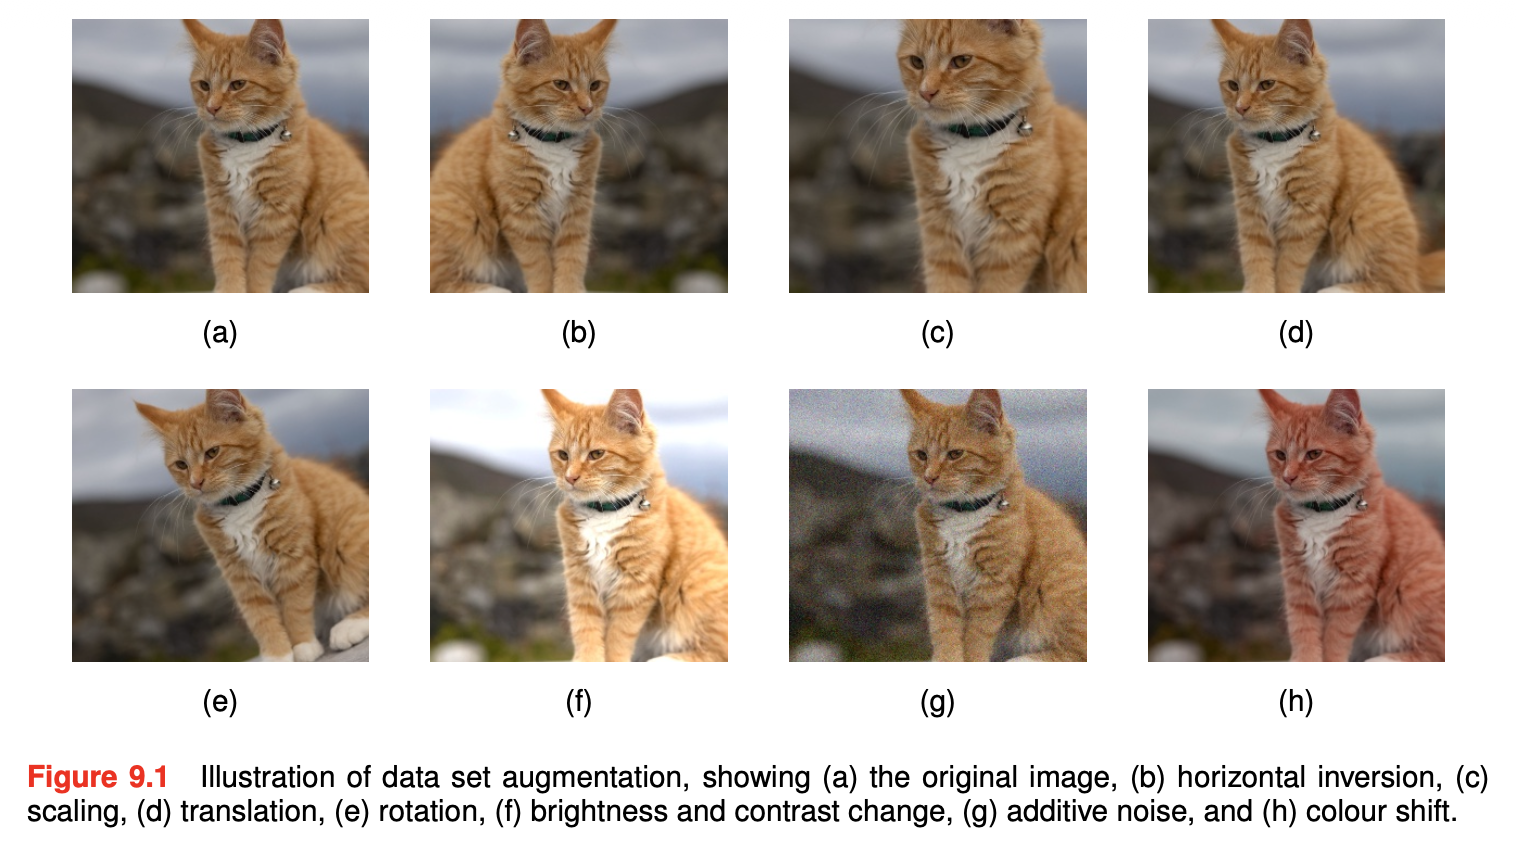
\includegraphics[width=\textwidth,height=0.5\textheight,keepaspectratio]{imgs/bishop_example/8.png}
\begin{itemize}
  \item Reconhecimento de imagem, reconhecimento de fala: funciona 
\item OCR: cuidado (b e d, 6 e 9)
\end{itemize}
\end{frame}


\begin{frame}{Equivariância}
\centering
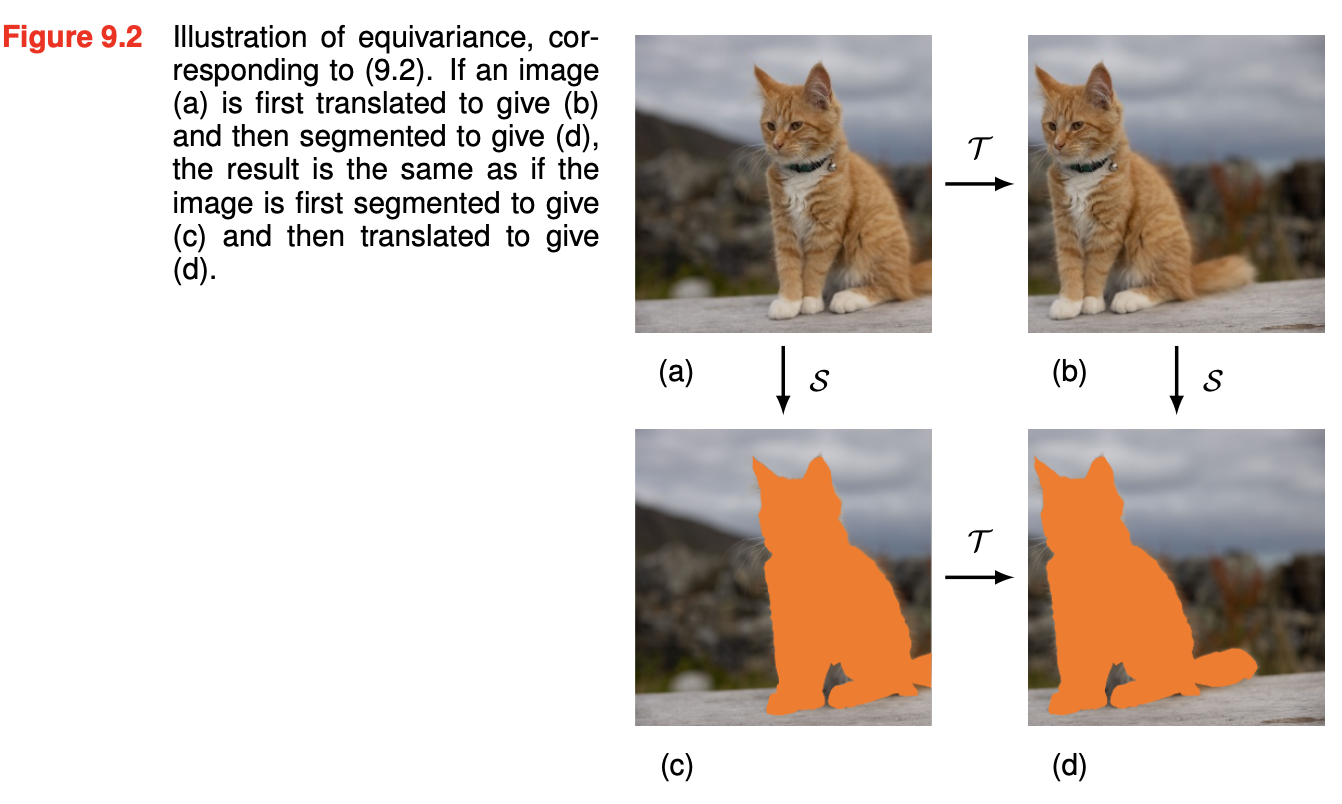
\includegraphics[width=\textwidth,height=0.7\textheight,keepaspectratio]{imgs/bishop_example/9.png}
\end{frame}


\section{Curvas de Aprendizado}

\begin{frame}{Convenção ``clássica'': Encerramento Antecipado}
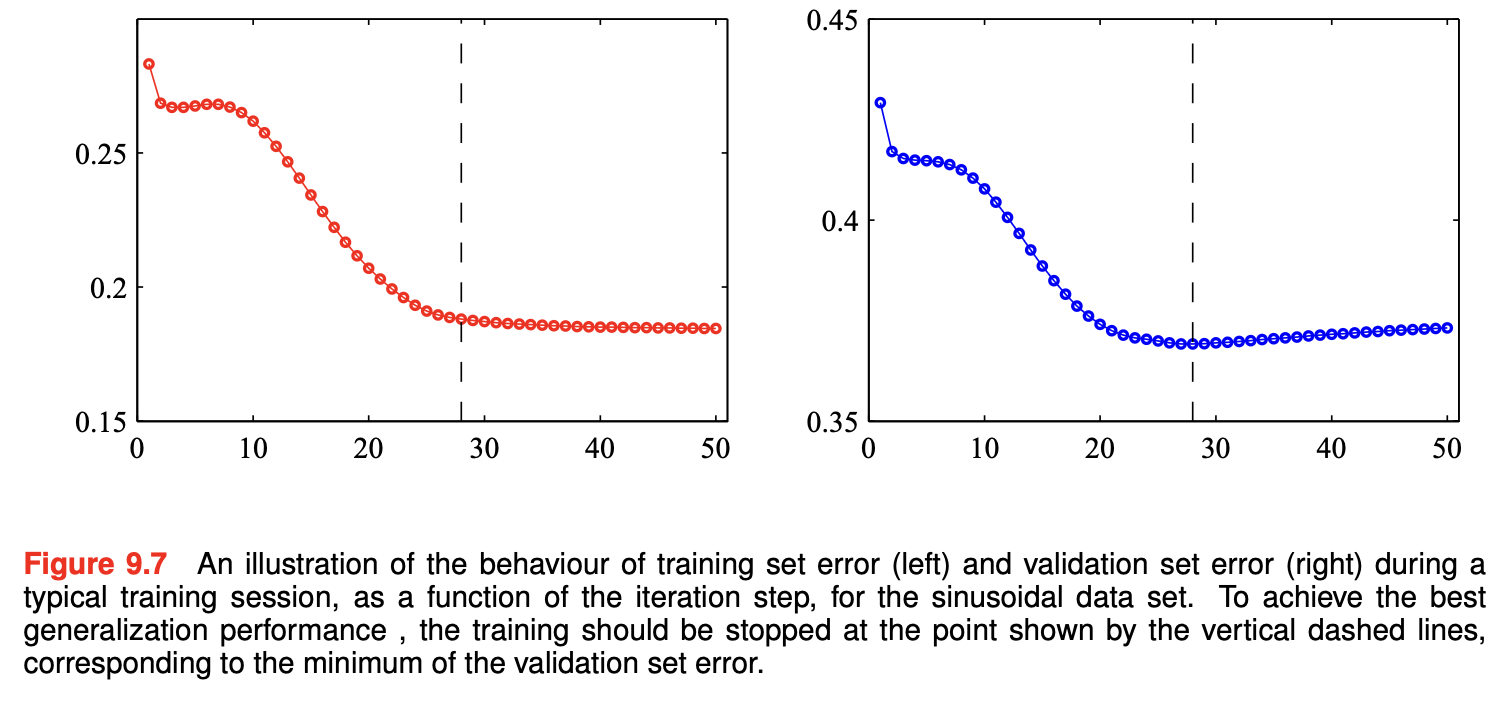
\includegraphics[width=\textwidth,height=0.5\textheight,keepaspectratio]{imgs/bishop_example/10.png}
\begin{itemize}
  \item \textbf{Trade-off Viés-Variância:}
    \begin{itemize}
      \item Poucos parâmetros: erro de teste alto (viés alto)
      \item Mais parâmetros: erro de teste diminui
      \item Parâmetros demais: erro de teste aumenta novamente (alta variância)
    \end{itemize}
\end{itemize}
\textbf{Crença clássica:} número de parâmetros deve ser limitado ao tamanho do conjunto de dados
\end{frame}

\begin{frame}{Convenção ``moderna'': \textbf{Double Descent}} 
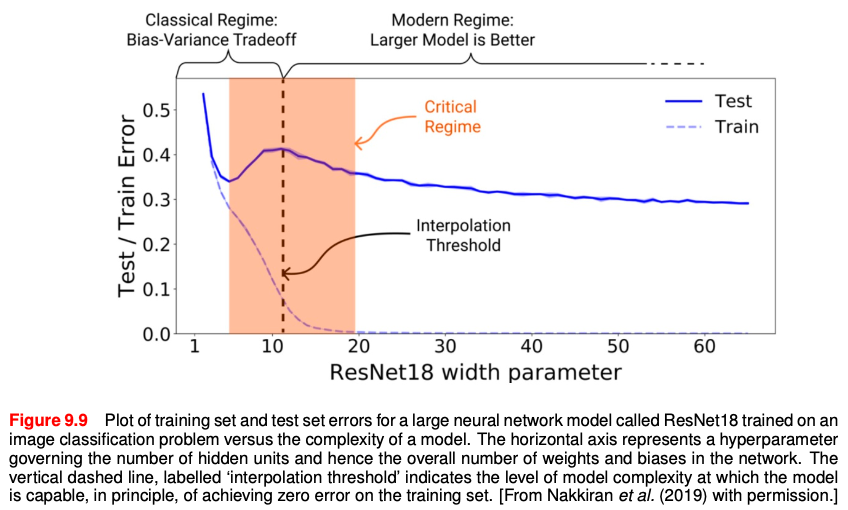
\includegraphics[width=\textwidth,height=0.5\textheight,keepaspectratio]{imgs/bishop_example/11.png}
  \begin{itemize}
  \item \textbf{Redes profundas:} bom desempenho mesmo quando a quantidade de parâmetros excede em muito o necessário para ajustar aos dados de treinamento 
\end{itemize}
\end{frame}

\begin{frame}{Convenção ``moderna'': \textbf{Double Descent}} 
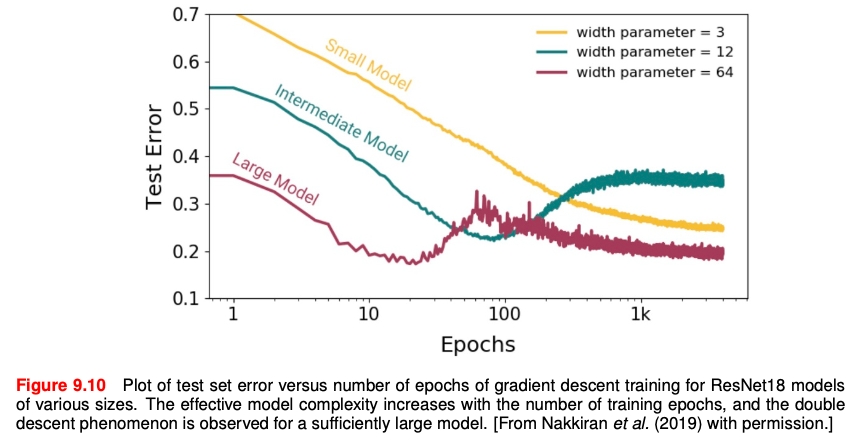
\includegraphics[width=\textwidth,height=0.7\textheight,keepaspectratio]{imgs/bishop_example/12.png}
    \tiny{Complexidade efetiva do modelo: quantidade máxima de dados de treinamento tal que o modelo atinja erro zero (limiar de interpolação). Dali em diante, a descendência dupla ocorre quando a complexidade do modelo excede esse limiar.}
\end{frame}


\section{Outras Formas de Regularização}
\begin{frame}{Batch Normalization}
\end{frame}

\begin{frame}{Bagging e Ensemble de Modelos}
\end{frame}


\begin{frame}{Aprendizado Residual}
\end{frame}

\begin{frame}{Dropout}
\end{frame}


\begin{frame}{Semi-Supervised Learning}
\end{frame}

\begin{frame}{Multi-Task Learning}
\end{frame}


\begin{frame}{Adversarial Training}
\end{frame}


\section{Alguns Casos Práticos}
\begin{frame}{Alguns Casos Práticos}
\end{frame}
?

\section{Conclusão}

\begin{frame}{Conclusão}
\end{frame}

\begin{frame}{Referências}
  Bishop
  Goodfellow
\end{frame}

\end{document}
